\documentclass{beamer}
\usetheme{Warsaw}
\usepackage{ragged2e}
\usepackage{multimedia}
\usepackage{polski}
\usepackage[utf8]{inputenc}
\usecolortheme{beaver}
\title[]
{Komputerowe modelowanie i rozwiązywanie łamigłówek geometrycznych wymagających detekcji kolizji}
\author[]
{
    promotor: dr Przemysław ~Kobylański\\
    autor: Tomasz ~Kulik
}
\institute[Politechnika Wrocławska]
{
  Wydział Podstawowych Problemów Techniki\\
  Politechnika Wrocławska\\
  Polska
}
\date[2017]
{2017}
\subject{Informatyka}


\begin{document}
    \begin{frame}
        \titlepage
    \end{frame}
    \begin{frame}
    	\frametitle{Założenia aplikacji}
        \begin{itemize}
            \item Aplikacja służy do rozwiązywania pewnego podzbioru łamigłówek logicznych składających się z 					połączonych mniejszych elementów.
            \item Rozwiązanie jest przedstawiane w formie animacji komputerowej.
        \end{itemize}
    \end{frame}
    \begin{frame}
    	\frametitle{Przykładowa układanka przed rozwiązaniem}
   		\centering
   		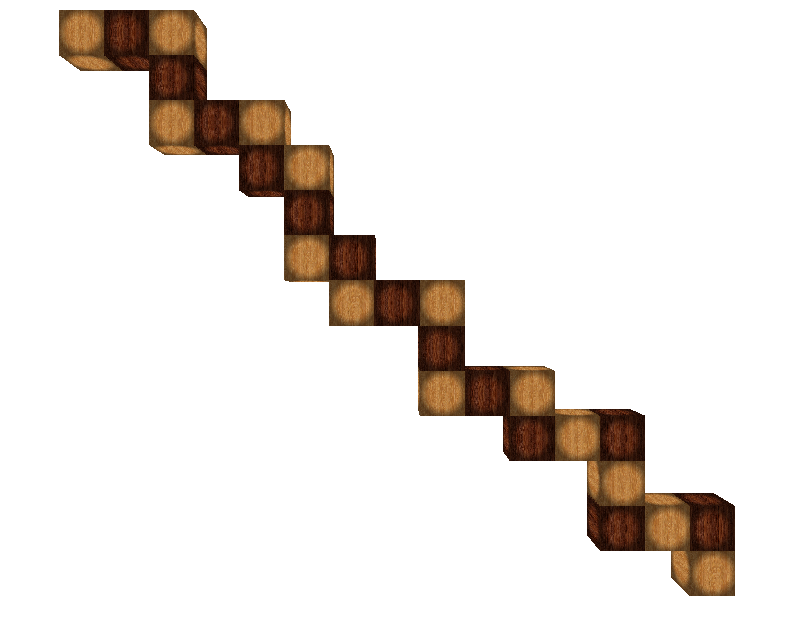
\includegraphics[width=0.6\textwidth]{play.png}
    \end{frame}

    \section{Reprezentacja modelu}
    \begin{frame}
    	\frametitle{Następny rozdział}
        \tableofcontents[currentsection]
    \end{frame}
    \begin{frame}
    	\frametitle{Przedstawienie problemu}
        \begin{itemize}
            \item Problem opisany jest jako wektor liczb naturalnych
            \item Każda liczba reprezentuje długość kolejnych fragmentów zagadki
            \item Między kolejnymi fragmentami znajdują się łączenia znaczące
        \end{itemize}
    \end{frame}
    \begin{frame}
    	\frametitle{Przedstawienie problemu}
        \begin{itemize}
            \item Opis spodziewanego rozwiązania przedstawiony jest w postaci ograniczeń w przestrzeni - 						sześcian o zadanej długości boku
            \item Program znajduje kobminację ruchów, jaką należy wykonać by rozwiązać łamigłówkę.
        \end{itemize}
    \end{frame}

    \section{Wykrywanie kolizji}
    \begin{frame}
        \frametitle{Następny rozdział}
        \tableofcontents[currentsection]
    \end{frame}
    \begin{frame}
    	\frametitle{Przewidywanie kolizji}
        \begin{itemize}
            \item Poszczególne elementy w modelu mogą obracać się względem siebie.
            \item Nie każdy obrót jest dozwolony - inny element może stać na przeszkodzie.
            \item Wymagane jest wykrycie potencjalnych kolizji celem wykluczenia danego ruchu.
        \end{itemize}
    \end{frame}
    \begin{frame}
    	\frametitle{Przewidywanie kolizji}
        	Wykrywanie kolizji pozwala uniknąć sytuacji, w której algorytm rozwiazujący będzie
        	próbował wykonać ruch niemożliwy do wykonania w realnym świecie (przeniknąć jeden obiekt
       		przez drugi).
    \end{frame}

    \section{Moduł rozwiązujący}
    \begin{frame}
    	\frametitle{Następny rozdział}
        \tableofcontents[currentsection]
    \end{frame}
    \begin{frame}
    	\frametitle{Podstawowe założenia}
        \begin{itemize}
            \item Model składa się z połączonych ze sobą elementów.
            \item Każde połączenie znaczące jest opisane jako stan opisujący względne położenie dwóch 							sąsiadujących fragmentów.
            \item Stany są reprezentowane jako liczby całkowite - ich ilość powinna być ograniczona w celu 						optymalizacji czasu wykonywania programu.
            \item Stan modelu w danej chwili można opisać jako wektor stanów połączeń znaczących.
        \end{itemize}
    \end{frame}
    \begin{frame}
    	\frametitle{Faza pierwsza}
        Znalezienie wektora stanów, który spełnia założenia celu.\\
        Algorytm ,,zwijający'' model:
        \begin{itemize}
            \item W kolejnych krokach manipuluje kolejno wybieranymi łączeniami i sprawdza czy wektor stanów 						obcięty od początku do aktualnego elementu spełnia założenia rozwiązania.
            \item Nie zważa na kolizje - jego celem jest jak najszybsze znalezienie końcowego wektora stanów.
        \end{itemize}
    \end{frame}
    \begin{frame}
    	\frametitle{Faza druga}
        \begin{itemize}
        	\item Posiadając końcowy wektor stanów algorytm w fazie drugiej manipuluje obrotami elementów, aby znaleźć kombinację ruchów rozwiązujących łamigłówkę.\\
        	\item Druga faza algorytmu respektuje wykrywane kolizje unikając ich w czasie poszukiwań docelowej 					kombinacji ruchów.
		\end{itemize}
    \end{frame}

    \section{Prezentacja wyniku}
    \begin{frame}
		\frametitle{Następny rozdział}
        \tableofcontents[currentsection]
    \end{frame}
    \begin{frame}
    	\frametitle{Animacja 3D}
        Moduł graficzny na podstawie otrzymanego wektora ruchów generuje trójwymiarową animację.\\
        Użytkownik może dowolnie obracać układankę, powiększać ją bądź pomniejszać.
    \end{frame}
    \begin{frame}
    	\frametitle{Animacja 3D}
    	\centering
    	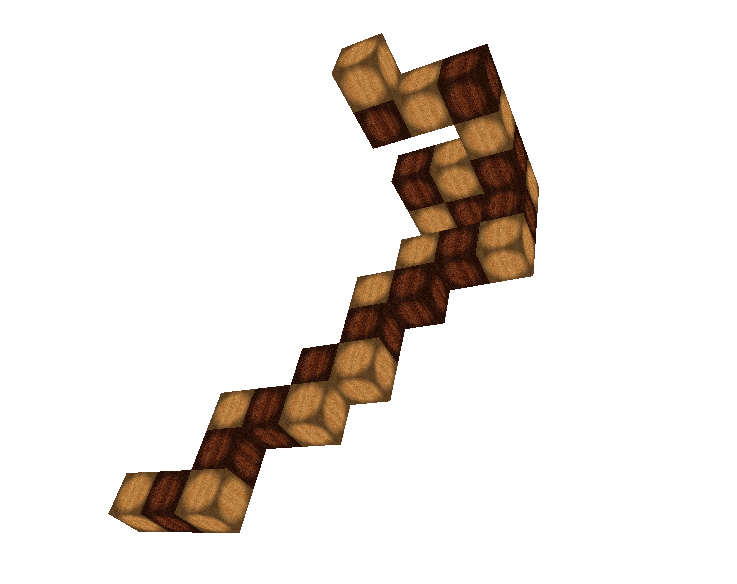
\includegraphics[width=0.6\textwidth]{using.png}
    \end{frame}
    \begin{frame}
        Dziękuję za uwagę
    \end{frame}

\end{document}
